\section{Systémy PZS (Architektura PZS. Prvky PZS. Typy systémů PZS podle komunikace. Dvojitě vyvážená smyčka.)}

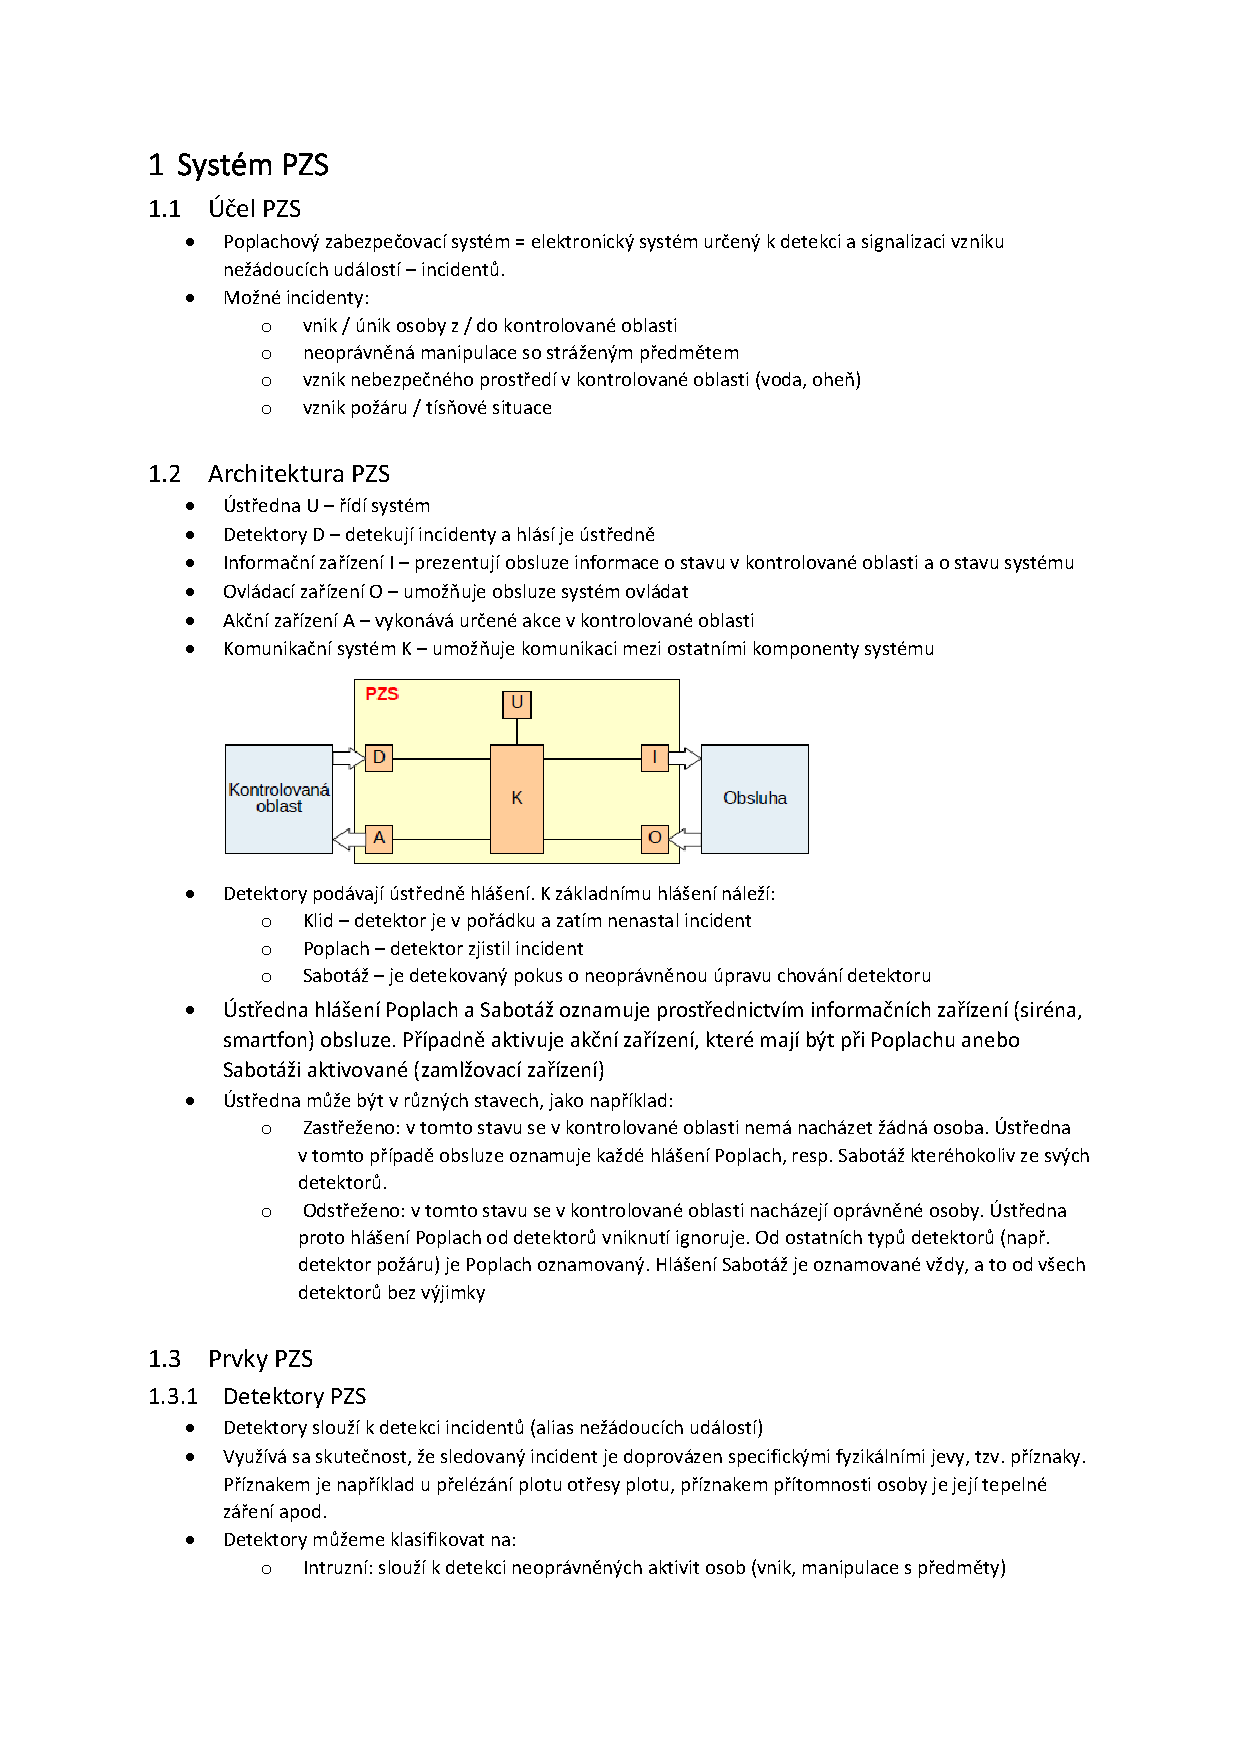
\includepdf[pages={1,2,3,4}]{BZSYstatnice.pdf}

\newpage
\section{Předmětové a překážkové detektory PZS (Typy detektorů z hlediska vícevrstvé ochrany. Typy předmětových detektorů\,--\,účel a jejich fyzikální princip. Typy překážkových detektorů\,--\,účel a jejich fyzikální princip. V rámci odpovědi vysvětlit i fungování piezoelektrického snímače, akcelerometru a tenzometru.)}

\includepdf[pages={5,6,7,8}]{BZSYstatnice.pdf}

\newpage
\section{Objemové a hraniční detektory PZS (Typy objemových detektorů\,--\,účel a jejich fyzikální princip. Typy hraničních detektorů\,--\,účel a jejich fyzikální princip. V rámci odpovědi vysvětlit i fungování pyroelektrického snímače.)}

\includepdf[pages={9,10,11,12}]{BZSYstatnice.pdf}

\newpage
\section[Dohledové videosystémy (Účel. Základní prvky. Schéma hybridního a digitálního systému. Architektura kamery. Kalkulace záběru. Techniky zpracování signálu\,--\,integrace snímků, BLC, WDR a HLC).]{Dohledové videosystémy (Účel. Základní prvky. Sché-ma hybridního a digitálního systému. Architektura kamery. Kalkulace záběru. Techniky zpracování signálu\,--\,integrace snímků, BLC, WDR a HLC).}

\includepdf[pages={13,14,15}]{BZSYstatnice.pdf}

\newpage
\section{Systémy EPS a hlásiče EPS (Účel. Architektura. Základní prvky. Schéma a princip fungování smyčkového a sběrnicového systému. Bodové hlásiče a~jejich fyzikální principy. Lineární hlásiče a jejich fyzikální principy. Prostorové hlásiče a jejich fyzikální principy.)}

\includepdf[pages={16,17,18,19}]{BZSYstatnice.pdf}

\newpage
\section{Systémy EKV (Účel, prvky a architektura systému EKV. Typy autentizace\,--\,princip a vlastnosti. Karty s magnetickým páskem\,--\,princip a vlastnosti. Bezkontaktní karty podle ISO 14443\,--\,princip a vlastnosti.)}

\includepdf[pages={20,21,22}]{BZSYstatnice.pdf}

\newpage
\section[Biometrické systémy EKV (Architektura a správa biometrického systému EKV. Autentizace otisky prstů, cévním řečištěm prstu a dlaně, obličejem a duhovkou\,--\,principy a vlastnosti.)]{Biometrické systémy\,EKV\,(Architektura\,a\,správa biometrického systému EKV. Autentizace otisky prstů, cévním řečištěm prstu a dlaně, obličejem a duhovkou\,--\,principy a vlastnosti.)}

\includepdf[pages={23,24,25}]{BZSYstatnice.pdf}

\newpage
\section{Systémy na ochranu zboží (Účel a klasifikace. Kabelové systémy\,--\,princip a vlastnosti. AM systémy\,--\,princip a vlastnosti. RF systémy\,--\,princip a vlastnosti.)}

\includepdf[pages={26,27}]{BZSYstatnice.pdf}

\newpage
\section{Elektronické platební systémy (Účel. Typy a jejich charakteristika. Vysvětlit protokol TLS. Vysvětlit nespřažený platební protokol.)}

\includepdf[pages={28,29}]{BZSYstatnice.pdf}

\newpage
\section{Ochrany digitálních děl (Účel a klasifikace ochran. Vzdálené DRM ochrany\,--\,typy, principy a vlastnosti. Lokální DRM ochrany\,--\,typy, principy a vlastnosti.)}

\includepdf[pages={30,31}]{BZSYstatnice.pdf}